\documentclass{article}
\author{Victor Mittermair, 11809916}
\usepackage{hyperref}
\usepackage{fancyhdr}
\usepackage{tikz} 
\usepackage{amsthm}
\usepackage{verbatim}
\usepackage{subfigure}
\usepackage{amssymb}
\usepackage{mathtools}
\usepackage{amsmath}
\usepackage{soul}
\usepackage{algorithm}
\usepackage{algpseudocode}
\usepackage{algorithmicx}
\usepackage{enumerate}

\newtheorem*{theorem}{Theorem}
\newtheorem*{lemma}{Lemma}
\theoremstyle{definition}
\newtheorem*{definition}{Definition}
\theoremstyle{remark}
\newtheorem*{remark}{Remark}
\newtheorem*{note}{Note}
\newtheorem*{statement}{Statement}
\newtheorem*{example}{Example}

%\lhead{\includegraphics[width=0.2\textwidth]{nyush-logo.pdf}}
\fancypagestyle{firstpage}{%
  \lhead{TU Vienna}
  \rhead{
  Discrete Math for Informatics WS 2022}
}

%%%% PROJECT TITLE
\title{Discrete Math for Informatics\\
        \Large \emph{6th Lecture}}


\date{\today} %NO DATE

\begin{document}
\maketitle
\thispagestyle{firstpage}

\begin{comment}
\section*{Graph}
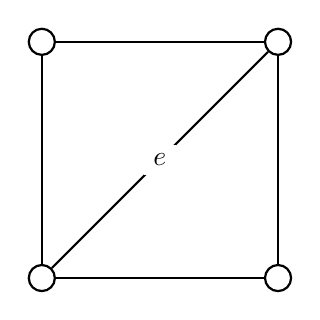
\begin{tikzpicture}[node distance={30mm}, thick, main/.style = {draw, circle}]
    \centering
    \node[main] (1)              {}; 
    \node[main] (2) [right of=1] {};
    \node[main] (3) [below of=1] {}; 
    \node[main] (4) [right of=3] {};
    \draw (1) -- (2) ; 
    \draw (1) -- (3); 
    \draw (2) -- (4); 
    \draw (3) -- (4);
    \draw (3) -- (2) node [midway, fill=white] {$e$}; 
\end{tikzpicture}
\end{comment}
\subsection*{Hamiltonian Graphs}
\begin{definition}
  A graph is \textbf{hamiltonian} if it contains a hamiltonian cycle, which is a cycle which visits every vertex exactly once.
\end{definition}
\begin{remark}
  It is NP-hard to find a hamiltonian cycle.
\end{remark}
\begin{definition}
  $G=(V,E)$ a graph, and let $[G]=(V,\widetilde{E})$ with $E_1:=E, E_{i+1}:=E_i\cup \{e=(u,v) \notin E | d(u) + d(v) \geq |V|\}$\\
  $\widetilde{E}$ is the set $E_k$ s.t. $d(u) + d(v) < |V|$ for all $(u,v) \notin E_k$
\end{definition}
\begin{theorem}
  $G$ is hamiltonian $\Leftrightarrow [G]$ is hamiltonian.
\end{theorem}
\begin{proof}
  $"\Rightarrow"$ $[G]$ is $G$ with some morde edges.\\
  $"\Leftarrow"$ suppose $H$ is a hamiltonian cycle in $[G]$, but $G$ is not hamiltonian,\\ $\Rightarrow \exists e=(u,v) \in E([G]) \backslash E(G)$ which is in every hamiltonian cycle of $[G]$ \\
  $\Rightarrow d_G(u)+d_G(v) \geq |V|$ because
  TODO: add picture
\end{proof}
\begin{remark}[Corollary]
  $|V| \geq 3, d(u)+d(v) \geq |V| \forall u,v \in V \Rightarrow G$ is hamiltonian (Ore 1960)\\
  $d(v) \geq \frac{|V|}{2} \forall v \in V \Rightarrow$ G is hamiltonian (Dirac 1952)
\end{remark}
\section*{Planarity}
\begin{definition}
  A graph is planar if there is a drawing of $G$ in $\mathbb{R}^2$ s.t. no two edges intersect (except at vertices).
\end{definition}
\begin{example}
  TODO: find planar graphs
\end{example}
\begin{theorem}
  TODO: find pictures of $K_{3,3}$ (complete bipartite graph) and $K_5$ are not planar.
\end{theorem}
\begin{definition}
  A \textbf{face} of a drawing of a graph is a region bounded by edges.
\end{definition}
\begin{theorem}[Euler's polyhedran formula]
  $|V|-|E|+|F|= 2$ for any drawing of a planar connected graph.
\end{theorem}
\begin{proof}
  induction on $|F|$: $|F|= 1$: $G$ is a tree $\Rightarrow$  $|V| - |E| + |F| = 2$\\
  $|F| > 1: \exists e$ bounding two faces, let $G^\prime = G \backslash e\\ \Rightarrow |V^\prime| = |V|, |E^\prime| = |E| - 1,|F^\prime|=|F|-1$\\
  $2 = |V^\prime|-|E^\prime|+|F^\prime| = |V| - |E|+1 + |F|-1$
\end{proof}
\begin{lemma}
  $G$ simple planar connected graph and every edge bounds two faces, then $|E| \leq 3|V|-6$ and if $G$ additionally has no triangles then $|E|\leq 2|V|-4$
\end{lemma}
\begin{proof}
  $f_j:= |\{f \text{a face with $j$ bounding edges}\}|\\
  \Rightarrow |F| = \sum_{j\geq 3}f_j$ \\
  $3|F| \leq \sum_{j\geq 3}jf_j = 2|E|$\\
  $0 = 3|V|-3|E|+3|F|-6 \leq 3|V|-3|E|+2|E|-6=3|V|-|E|-6$\\
  if no triangles\\
  $4|F|\leq 2|E|\\
  0=2|V|-2|E|+2|F|-4 \leq 2|V|-2|E|+|E|-4=2|V|-|E|-4$
\end{proof}
\begin{remark}[Corollary]
  $K_{3,3}$ is not planar: no triangles and  $|V| = 6, |E|=9$\\
  $K_5$ is not planar $|V|=5, |E|=10$
\end{remark}
\begin{theorem}[Kuratowski-Wagner]
  $G$ is planar if and only if $G$ has no subgraph which is a subdivision of $K_{3,3}$ or $K_5$
\end{theorem}
\end{document}